\documentclass[12pt,a4paper]{article}
\usepackage[utf8]{inputenc}
\usepackage[ukrainian]{babel}
\usepackage{indentfirst}
\usepackage{misccorr}
\usepackage{graphicx}
\graphicspath{{pictures/}}
\DeclareGraphicsExtensions{.jpg, .eps}
\usepackage{amsmath}
\usepackage{setspace}  
\onehalfspacing

\begin{document}
	\begin{center}
		\section*{Постановка задачі математичного програмування}
	\end{center}
\begin{flushleft}
\parbox{14,5 cm}{\parindent=1 cm  \newtheorem{law}{Означення}\newtheorem{law1}[law]{Означення}\newtheorem{law2}[law]{Означення} \newtheorem{law3}[law]{Означення}\newtheorem{law4}[law]{Означення} \newtheorem{theorem}{Теорема}
\newtheorem{consequence}{Наслідок} \newtheorem{consequence1}[consequence]{Наслідок} \newtheorem{theorem1}[theorem]{Теорема} \newtheorem{law5}[law]{Означення} \newtheorem{theorem2}[theorem]{Теорема} \newtheorem{theorem3}[theorem]{Теорема}
\begin{law}
Точка ${x}^*\in R$ називається точкою глобального мінімуму функції $\varphi \left(x\right)$ на множині $R$, якщо 
\begin{displaymath}
\varphi \left({x}^*\right) \le \varphi \left(x\right) \ \forall \ x \in R. 
\end{displaymath}
 Множину точок глобального мінімуму функції позначимо через ${X}_*$ 
\end{law}
\begin{law1}
Точка ${x}^*\in R$ називається точкою локального мінімуму функції $\varphi \left(x\right)$ на множині $R$, якщо знайдеться константа $\varepsilon > 0$ така, що
\begin{displaymath}
\varphi \left({x}^*\right) \le \varphi \left(x\right) \ \forall \ x \in R, \text{ що задовольняють умові }\left \| x-{x}^*\right \| \le \varepsilon.
\end{displaymath}
\end{law1}
\begin{law2}
Точка ${x}^*\in R$ називається точкою строгого мінімуму (в локальному чи глобальному сенсі), якщо відповідні нерівності в наведених означеннях виконуються як строгі (при $x \neq {x}^*$)
\end{law2}}
\end{flushleft}
\begin{flushleft}
\parbox{14,5 cm}{\parindent=1 cm  Аналогічно вводяться означення точок локального і глобального максимуму.}
\end{flushleft}
\begin{flushleft}
\parbox{14,5 cm}{\parindent=1 cm  Умовне позначення $\varphi\left(x\right)\rightarrow extr, x\in R$ застосовується при розгляданні задачі пошуку екстремуму функції $\varphi\left(x\right))$ на множині $R$. Запис
\begin{displaymath}
\varphi\left(x\right)\rightarrow min \text{ або } \varphi\left(x\right)\rightarrow max
\end{displaymath}
означає, що досліджується тільки задача мінімізації або максимізації функції $\varphi\left(x\right)$.}
\end{flushleft}
\begin{flushleft}
\parbox{14,5 cm}{\parindent=1 cm  Так як довільна задача максимізації функції $\varphi\left(x\right)$ може бути записана у вигляді задачі мінімізації функції $-\varphi\left(x\right)$, то всі теоретичні міркування можна проводити тільки для задачі на мінімум.}
\end{flushleft}
\begin{flushleft}
\parbox{14,5 cm}{\parindent=1 cm  \textbf{Приклад.} Розглянемо функцію 
\begin{displaymath}
\varphi\left(x\right) = \left\{ \begin{array}{ll}
{x}^2+3, & x\in\left[-2;1\right],\\
4, & x\ge 1
\end{array} \right.
\end{displaymath}}
\end{flushleft}
\begin{figure}[hb!]
\center{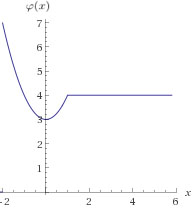
\includegraphics[width=4cm, height=4cm]{1}}
\end{figure}
\begin{flushleft}
\parbox{14,5 cm}{\parindent=1 cm  Ця функція на $\left [-2; +\infty \right )$ має одну точку строгого глобального мінімуму ${x}^*=0$, $\min\limits_{x \in R}{\varphi\left(x\right)}=\varphi\left(0\right)=3$. Точка ${x}^*=-2$ є точкою строгого локального максимуму, $\varphi\left({x}^*\right)=\varphi\left(-2\right)=7$. Промінь $\left [1; +\infty \right )$ - є множина нестрогого максимуму, $\max {\varphi\left(1\right)}=4$.}
\end{flushleft}
\begin{flushleft}
\parbox{14,5 cm}{\parindent=1 cm   \textbf{Приклад.} Функція $\varphi\left(x\right)={e}^{-x}$, $R = \left\{ x \in {E}^1 | x\ge 0\right\}$ має одну точку строгого глобального максимуму ${x}^*=1$ і не має точок мінімуму.}
\end{flushleft}
\begin{flushleft}
\parbox{14,5 cm}{\parindent=1 cm  \textbf{Приклад.}  Функція $\varphi\left(x\right)=x$ не досягає екстремуму ні в одній точці множини $R = \left\{ x \in {E}^1 | 2 < x < 3 \right\}$}
\end{flushleft}
\begin{figure}[h!]
\center{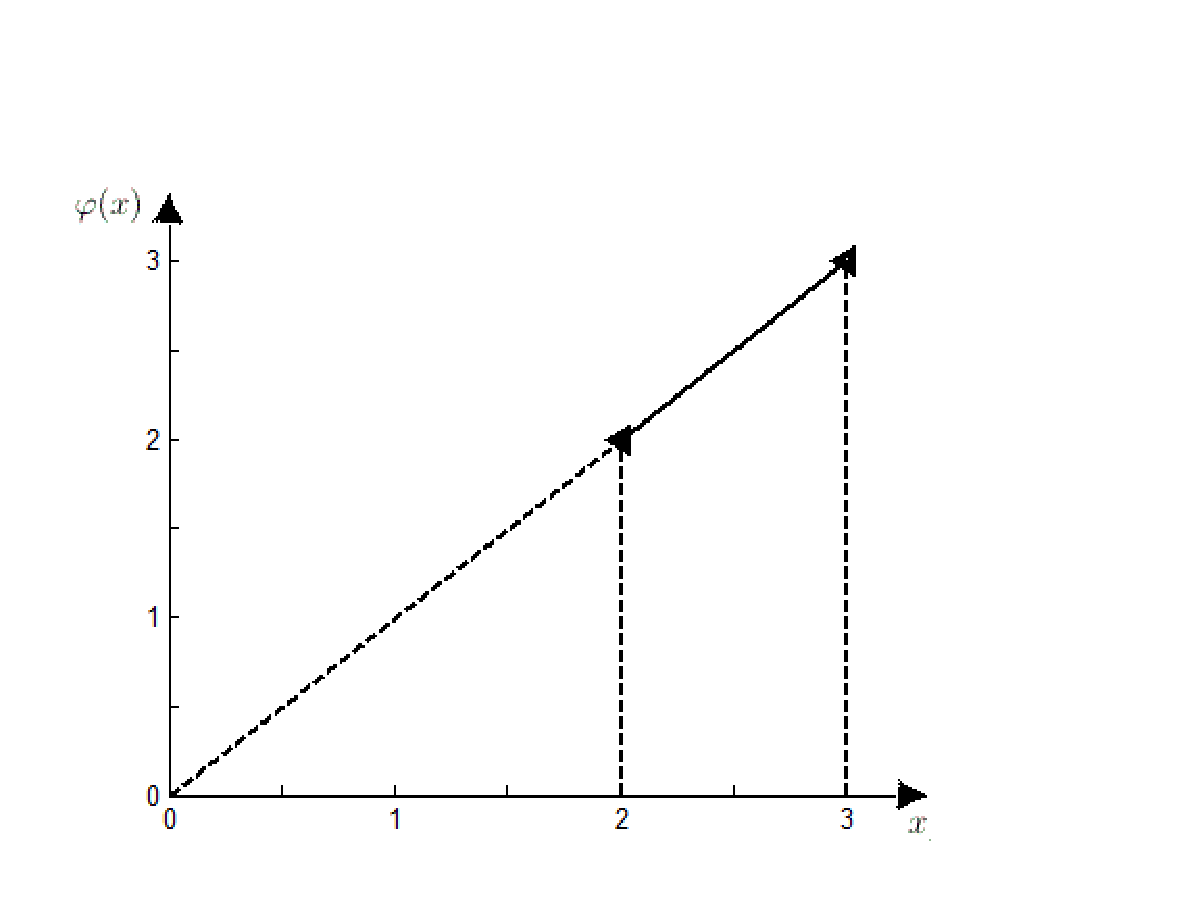
\includegraphics[width=7cm, height=5cm]{2}}
\end{figure}
\begin{flushleft}
\parbox{14,5 cm}{\parindent=1 cm Узагальненням поняття найменшого значення функції є визначення нижньої межі.}
\end{flushleft}
\begin{law3}
Нехай функція $\varphi\left(x\right)$ обмежена знизу на множині $R$. Число ${\varphi}_*$ називається нижньою межею (інфімумом) $\varphi\left(x\right)$, якщо воно є найбільшим з нижніх меж функції $\varphi\left(x\right)$ на $R$, тобто
\begin{enumerate}
\item $${\varphi}_* \le \varphi \left(x\right) \ \forall \ x \in R,$$
\item $$\forall \varepsilon > 0\  \exists \ {x}_\varepsilon \in R: \varphi\left({x}_\varepsilon\right) < {\varphi}_* + \varepsilon.$$
\end{enumerate}
\end{law3}
\begin{flushleft}
\parbox{14,5 cm}{\parindent=1 cm Якщо функція $\varphi\left(x\right)$ обмежена знизу на $R$, то існує єдина скінчена нижня межа цієї функції на множині $R$. Приймаючи у якості інфімуму необмеженої знизу на $R$ функції ${\varphi}_* = -\infty$, можна вважати, що нижня межа (на відміну від мінімуму) існує завжди.}
\end{flushleft}
\begin{flushleft}
\parbox{14,5 cm}{\parindent=1 cm  Аналогічно вводиться поняття верхньої межі (супремуму), як найменшої верхнбої межі функції $\varphi\left(x\right)$ на $R$.}
\end{flushleft}
\begin{center}
		\subsection*{Збіжність в екстремальних задачах. Існування екстремумів}
	\end{center}
\begin{flushleft}
\parbox{14,5 cm}{\parindent=1 cm Розглянуті приклади показують, що не завжди існує точка, в якій досягається нижня межа цільової функції. Тому краще розглянути узагальнену задачу оптимізації - побудову мінімізуючої послідовності.}
\end{flushleft}
\begin{law4}
Послідовність точок $\left\{ {x}^k\right\}$ з припустимої множини $R$ називається мінімізуючою для функції $\varphi\left(x\right)$, якщо $$\lim_{k\rightarrow\infty}{\varphi\left({x}^k\right)}=\inf_{x\in R}{\varphi\left(x\right)}={\varphi}_*$$
\end{law4}
\begin{flushleft}
\parbox{14,5 cm}{\parindent=1 cm Побудова мінімізуючих послідовностей є метою розв'язування задачі мінімізації не тільки в тому випадку, коли точна нижня межа функції не досягається. Більшість методів оптимізації генерують послідовність точок, яка є мінімізуючою.}
\end{flushleft}
\begin{flushleft}
\parbox{14,5 cm}{\parindent=1 cm Розглянемо достатню умову досягнення верхньої і нижньої меж.}
\end{flushleft}
\begin{theorem}[Вейєрштрасса]\label{thVeyer}
Нехай $R$ - обмежена і замкнута множина, функція $\varphi\left(x\right)$ - неперервна на  $R$. Тоді ${f}_*=\inf\limits_{x \in R}{\varphi\left(x\right)}>-\infty$, множина точок глобального мінімуму непуста, обмежена і замкнута, а довільна мінімізуюча послідовність збігається до ${X}_*$.
\end{theorem}
\begin{consequence}
Нехай $R$ - непуста замкнута підмножина ${E}^n$, функція $\varphi\left(x\right)$ неперервна на $R$ і для деякої фіксованої точки ${x}^0$ множина Лебега $$L\left({x}^0\right) = \left\{ x\in R\ |\ \varphi\left(x\right)\le\varphi\left({x}^0\right)\right\}$$ обмежена. Тоді виконуються всі твердження теореми Вейєрштрасса при умові, що елементи мінімізуючої послідовності ${x}^k\in L\left({x}^0\right)$.
\end{consequence}
\begin{consequence1}
Нехай $R$ - непуста замкнута підмножина ${E}^n$, функція $\varphi\left(x\right)$ неперервна на $R$ і для довільної послідовності $\left\{ {x}^k\right\}$ точок з $R$, що задовільняють умові $\lim\limits_{k\rightarrow\infty}{\left\| {x}^k\right\|}=+\infty$, виконується співвідношення $\lim\limits_{k\rightarrow\infty}{\varphi\left({x}^k\right)}=+\infty$. Тоді виконуються всі твердження теореми Вейєрштрасса.
\end{consequence1}
\begin{flushleft}
\parbox{14,5 cm}{\parindent=1 cm Аналогічно формулюється теорема для задачі максимізації.}
\end{flushleft}
\begin{center}
\subsection*{Мінімізація функцій без обмежень}
\end{center}
\begin{flushleft}
\parbox{14,5 cm}{\parindent=1 cm Розглянемо задачу}
\end{flushleft}
\begin{equation}\label{extr}
\varphi\left(x\right)\rightarrow extr,\ x\in {E}^n
\end{equation}
\begin{flushleft}
\parbox{14,5 cm}{\parindent=1 cm Класичний підхід до пошуку безумовного екстремуму грунтується на таких твердженнях.}
\end{flushleft}
\begin{theorem1}[необхідна умова екстремуму першого порядку]
Нехай фнкція $\varphi\left(x\right)$ диференційована в точці ${x}^*\in {E}^n$. Тоді якщо ${x}^*$ - локальний розв'язок задачі \eqref{extr}, то 
\begin{equation}\label{partial}
\frac{\partial\varphi\left({x}^*\right)}{\partial x}=0
\end{equation}
\end{theorem1}
\begin{law5}
Розв'язки системи рівнянь \eqref{partial} називаються стаціонарними або критичними точками.
\end{law5}
\begin{theorem2}[необхідна умова екстремуму другого порядку]
Нехай фнкція $\varphi\left(x\right)$ двічі диференційована в точці ${x}^*\in {E}^n$. 
\begin{enumerate}
\item Якщо ${x}^*$ - точка локального мінімуму в задачі \eqref{extr}, то матриця $\frac{{\partial}^2\varphi\left({x}^*\right)}{\partial {x}^2}$ невід'ємно визначена, тобто $$\left(\frac{{\partial}^2\varphi}{\partial {x}^2} x, x\right)\ge 0\ \forall\ x\in {E}^n.$$
\item Якщо ${x}^*$ - точка локального максимуму, то матриця $\frac{{\partial}^2\varphi\left({x}^*\right)}{\partial {x}^2}$ недодатньо визначена, тобто $$\left(\frac{{\partial}^2\varphi}{\partial {x}^2} x, x\right)\le 0\ \forall\ x\in {E}^n.$$
\end{enumerate} 
\end{theorem2}
\begin{theorem3}[достатня умова екстремуму]
Нехай функція $\varphi\left(x\right)$ двічі диференційована в точці ${x}^*\in {E}^n$ і $\frac{\partial\varphi\left({x}^*\right)}{\partial x}=0$.
\begin{enumerate}
\item Якщо матриця $\frac{{\partial}^2\varphi\left({x}^*\right)}{\partial {x}^2}$ додатньо визначена, то ${x}^*$ - точка строгого локального мінімуму функції $\varphi\left(x\right)$ на ${E}^n$.
\item Якщо матриця $\frac{{\partial}^2\varphi\left({x}^*\right)}{\partial {x}^2}$ від'ємно визначена, то ${x}^*$ - точка строгого локального максимуму функції $\varphi\left(x\right)$ на ${E}^n$.
\end{enumerate} 
\end{theorem3}
\end{document}